\documentclass[letterpaper,12pt]{article}
\usepackage{amsmath}
\usepackage{float}
\usepackage[margin=1in]{geometry}
\usepackage{graphicx}
\usepackage{placeins}
\usepackage{siunitx}
\usepackage[title]{appendix}
\usepackage{pdflscape}
\usepackage{tabularx}
\usepackage{times}
\usepackage{url}


\begin{document}

\begin{titlepage}
    \begin{center}
        \vspace*{1cm}

        \Large
        \textbf{ELEC 390 Main Project: Accessible Electronics Instrumentation}

        \vspace{0.5cm}
        TeachEE\\
        Presented for ELEC 498\\
        Group 18 \\
        \vspace{1.5cm}
        \normalsize
        \textbf{John Giorshev (20103586, john.giorshev@queensu.ca) \\ Eric Yang (20120750, e.yang@queensu.ca) \\ Ethan Peterson (20105011, 17emp5@queensu.ca) \\ Timothy Morland (20096286, 17tm22@queensu.ca)}

        \vfill
            
        \textbf{Supervisors:}\\
        Dr. Sean Whitehall (sw109@queensu.ca) \\
        Dr. Thomas Dean (tom.dean@queensu.ca) \\
            
        \vspace{0.8cm}

        Date: \today \\~\\
        I confirm that the team has consulted me regarding the project and the
        material described in this proposal.\\
        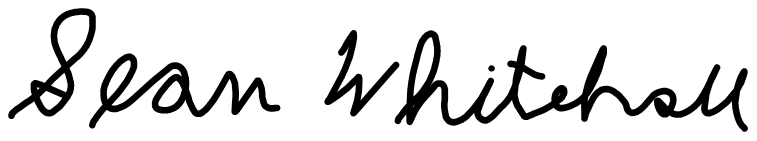
\includegraphics{figures/SWsignature} \\
        
\includegraphics{figures/TDsignature} \\
    \end{center}
\end{titlepage}
\section*{Abstract}
% 300 words max
The movement to online education and remote work has necessitated the need for a
new kind of electrical instrument. Students can no longer use the expensive
tools on university campuses for their engineering labs. As a result, professors
have had to send students individual lab kits that require curricular compromise
in the lab procedures.\\

\noindent
This report proposes a solution in the form of TeachEE, which combines the
signal generator and oscilloscope functionality into a cheap device specifically
for engineering labs. The impact of this device will be making available a cheap
oscilloscope that also provides a sophisticated software package. The result is
greater access to electronics for all students.\\

\noindent
There are five steps in the development of the solution. These consist of PCB
design, embedded code development, microcontroller driver code development, OS
driver code development, and application development. Development will begin on
September 1st and is scheduled for a mid-January finish to allow time for
testing of the prototype.

\newpage

\tableofcontents
\listoffigures
\listoftables
\newpage

% REPORT BODY (20 Page Max)
\section{Problem Description} \label{sec:prob-desc} % Ethan
Since the onset of the COVID-19 pandemic, universities and all other education
institutions have had quickly transition to an online mode of delivery. While
this new form of education has been an adjustment for all students it is
particularly difficult for engineers and other students partaking in programs
with an emphasis on hands-on lab activities. In the case of ECE students, the
most glaring compromise of online lab delivery is circuits labs and analyzing
circuits that have been constructed in the remote environment. Before the
pandemic, circuit data was collected using monolithic and expensive
oscilloscopes available to students in school lab spaces. These oscilloscopes
integrate display and processing functionality into one single device. While
efficient and effective in the lab environment, it is not economically possible
to send each individual student one of these instruments to complete their lab
work. The solution to this issue has been to use handheld oscilloscopes and
signal generators that lack the data capture functionality of their more
expensive counterparts. Additionally, this solution does not provide any means
of porting data from instrument to computer for calculations and analysis.\\

\noindent
This problem is endemic for both students and professors. Students find the
cheaper equipment harder to use in addition to requiring several separate power
outlets for the circuit, signal generator, and oscilloscopes. Professors must
make difficult decisions with regard to pairing down the scope of lab activities
since students can no longer effectively capture data from their physical
circuits.

\subsection{User Study}
Professor Sean Whitehall is an Electrical and Computer Engineering professor at
Queen's University. Dr. Whitehall teaches both ELEC 252 and ELEC 353 which
involve the construction and characterization of amplifier circuits. In the fall
2020 semester, Dr. Whitehall taught ELEC 353 remotely. In order to build
students' skills in the construction of physical circuits, Dr. Whitehall provided
lab kits to all students enrolled in the course. While the lab kits worked well,
students accidentally broke their signal generators through over-voltage and
labs had to be scaled down to accommodate the lesser instrumentation equipment.
Dr. Whitehall is supervising this capstone project and is interested in an
economic solution to the current pitfalls of remote lab work.


\section{Impact} % John

\subsection{Economic}

Unfortunately, proper economic evaluations of the oscilloscope market lay behind
massive paywalls \cite{paywalled_econ}. This necessitates the re-creation of
research which already exists, albeit, with a specialized scope and reduced
fidelity. The scope is reduced to the target market, which includes universities
with oscilloscope labs.\\

\noindent
At Queen's University there are approximately 19000 undergraduate students
\cite{queens_enroll_stats}. That gives $19000/4 \approx 5000$ students in each
year. ELEC 221 is the introduction to circuits class. As an approximation, it is
assumed that everyone who needs to use an oscilloscope takes that class. In the
Fall of 2019, there were 169 people enrolled in ELEC 221. This means that $169 /
5000 \approx 3\%$ of students require an oscilloscope.\\

\noindent
In 2019, there were 1.36 million students in Canada \cite{canada_students}.
Extrapolating 3\% of 1.36 million gives 40k undergraduate students in Canada
that require oscilloscopes.

\subsection{Cultural}

As discussed later in Section \ref{sec:existing-sol}, even the cheapest of
oscilloscopes are quite costly. The expectation is that an oscilloscope is a
bulky expensive tool which requires thousands of dollars to purchase. This
expectation is understandable since this type of oscilloscope is all that is
seen by the average person. TeachEE would change this norm, and re-brand what is
considered an average oscilloscope.

\subsection{Social}

Electronic hobbyists have diminished over the past 40 years. This is due to a
variety of factors, including: the growing complexity of the field, change in
economics due to cheap offshore manufacturing, and the failure of supporting
companies such as RadioShack \cite{elec_hobby}. The lack of simple cheap
oscilloscope certainly does not improve the vitality of the hobby. This product
will provide opportunity for more people, and will boost interest in the
electronics field in general.

\section{Solution} % Ethan
The proposed solution to the issue discussed in Section \ref{sec:prob-desc} is
called TeachEE, which stands for Teach Electrical Engineering. The TeachEE
bundles oscilloscope and signal generator functionality into a single device
that connects to the students' computer via USB. This USB connection takes care
of both power and data transmission. This allows students to work from their
computers without the need for several power outlets. The waveforms from the
TeachEE's input are displayed on the student's computer screen in a Graphical
User Interface (GUI) reducing hardware cost by avoiding the need for a display.
Moreover, all signal processing tasks are computed on the student's computer,
leveraging their powerful processors, thus keeping the compute resources on the
physical device as cheap as possible. Additionally, since the data is
sent to the computer for processing, it can also be exported from the GUI to an
excel format for students to use in their lab reports and analysis. The GUI on
the student's computer resolves problems with ease of use and data export. The
TeachEE will also resolve reliability issues by implementing both over-voltage
and over-current protections.

\subsection{Existing Solutions} \label{sec:existing-sol} There are two existing
solutions for this problem. The first existing solution is sending out lab kits
with discrete oscilloscopes and signal generators independent of the computer.
Section \ref{sec:prob-desc} discusses the issues with this approach in terms of
curricular limitations and reliability. The second existing solution are other
USB oscilloscopes. The most similar USB oscilloscope is the BitScope,
specifically the (cheapest) BS05U model \cite{noauthor_bitscope_nodate}. The
BitScope website shows it clearly targets the in-person lab environment
\cite{bitscope_education}. This device from BitScope performs a similar task in
having a GUI software and signal generator. However, the device is prohibitively
expensive to send to individual students at a cost of \$145 USD per unit. The
price is likely high due to the high sample rate and 20 Mhz bandwidth. While
this extra bandwidth is helpful when working with high speed signals on printed
circuit boards, all university labs where circuits are constructed on prototyping
boards by hand do not exceed 1 Mhz as indicated by Dr. Whitehall. Thus, the
extra bandwidth provided by the BitScope is not helpful in this context and
should be exchanged for a lower cost device. For example, the oscilloscopes sent to
students in the ELEC 353 circuits class at Queen's are less than half the cost
of the BitScope at \$46 USD on Amazon \cite{scope_353}.

\subsection{SWOT Analysis}
Table \ref{tab:swot} contains the SWOT analysis for TeachEE.

\begin{table}[h!]
    \centering
    \caption{SWOT Analysis Matrix}
    \begin{tabularx}{\textwidth}{X|X}
        Strengths & Weaknesses \\
        \hline
        \begin{itemize}
            \item Understanding of the needs of the educational market achieved
            by performing user interviews with Queen's ECE professors.
            \item Ability to minimize hardware cost by drawing on the
            computational power of computers that students already own.
            \item Understanding of students' needs due to being in the
            university environment.
        \end{itemize}
        &
        \begin{itemize}
            \item The device has the minimum feature set needed for Electronics
            labs and nothing more.
            \item The device will have lower bandwidth and sample rate in
            comparison to more expensive competitors.
        \end{itemize} \\
        \hline
        Opportunities & Threats \\
        \hline
        \begin{itemize}
            \item The current remote delivery of university classes presents an
            opportunity in marketing the device to secondary and post-secondary
            institutions alike.
            \item As remote work and education become normalized after the
            pandemic, demand will be greater for devices like TeachEE that help
            close the gap with in-person work.
        \end{itemize}
        &
        \begin{itemize}
            \item Other oscilloscope manufacturers compete in the education
            market in order to familiarize students with their technology. As
            such, universities are spoiled for choice in who they buy their
            instruments from.
            \item Competitors could see the TeachEE and aim to replicate its
            unique value proposition of accessible remote instrumentation.
        \end{itemize}
    \end{tabularx}
    \label{tab:swot}
\end{table}
\FloatBarrier

\section{Components and Design}
\subsection{Hardware} % Ethan
The physical TeachEE device will come in the form a custom Printed Circuit Board
(PCB) design. This PCB will power and provide debugger access
to a microcontroller through a USB connector. Additionally, the PCB will have a
BNC connector mounted on it for probe compatibility with other oscilloscopes.
The connector will be connected to the Analog to Digital Converter (ADC) of the
microcontroller. A second BNC connector is provided for the signal generator
output which will be connected to the Digital to Analog Converter (DAC) on the
microcontroller. A system block diagram representation of the PCB is given in
Figure \ref{fig:block-diagram-pcb}.

\begin{figure}[h!]
    \centering
    \caption{System Block Diagram of the TeachEE PCB. Note that ``MCU'' represents the microcontroller.}
    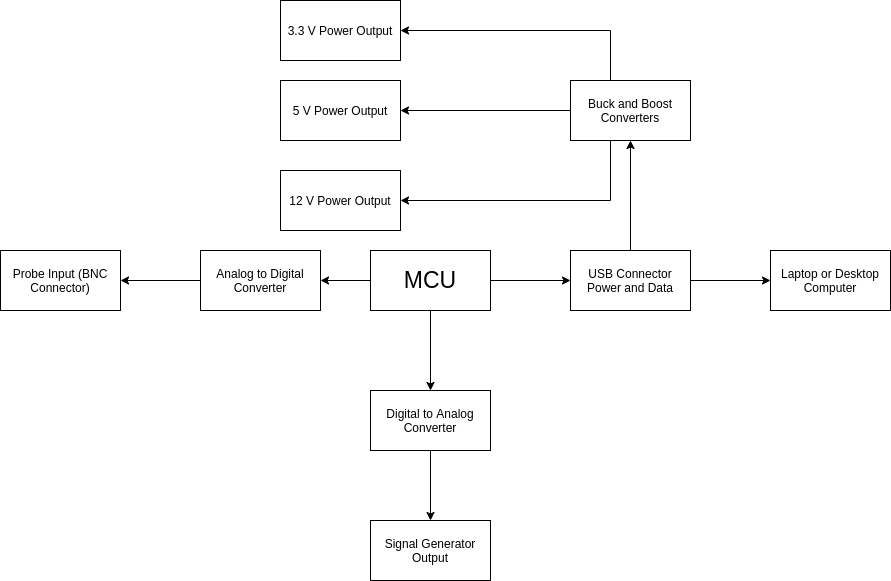
\includegraphics[width=\textwidth]{figures/pcb-block-diagram.png}
    \label{fig:block-diagram-pcb}
\end{figure}
\FloatBarrier

\noindent
As shown in the figure above, the USB connector not only powers the
microcontroller (MCU) but also connects ``buck'' and ``boost'' circuitry to
provide the student with different output supply voltages. The 5V output is
created directly from the 5V provided over USB. The 3.3V output is made using
the buck converter circuit to step down the voltage from 5 to 3.3 V. A linear
regulator solution could also be used here since the voltage drop is small but
the use of a buck converter will allow students to drive their circuits with
more current without heating the TeachEE as rapidly. It should be noted that the
ability to drive higher current circuits is dependent on the power rating of the
USB port the device is connected to. By default, the TeachEE will have a current
of 500 mA as per the USB specification \cite{kollman_powering_2002}. However,
the student could choose to override this and go higher, it is in these cases
where a buck topology is essential. The 12V output is produced via boost
converter circuit which will take the 5V supply from USB and boost it 12 V at
the cost of current draw capability.

\subsection{Software} % Eric and John
\subsubsection{Firmware} % Eric
% Voltage sampling code
% Signal generator code
The firmware running on the microcontroller will be written in C. It will take
inputs from two sources: the oscilloscope probes and the microcontroller driver.
It will sample voltages measured by the oscilloscope probes and pass it to the
driver. By offloading all signal processing to the desktop or laptop computer,
the firmware can be made very lightweight and fast, reducing microcontroller
resource usage. The firmware will also be responsible for setting signal
generator settings, such as signal frequency, signal amplitude, and DC offset.
These settings will be communicated from the application whenever the user
supplies the signal generator parameters through the user interface.

\subsubsection{Drivers} % John
% Include drivers on both sides

The driver on the user's computer will be written using Microsoft's kernel-Mode
Driver Framework (KMDF) via Visual Studio. The driver must be a kernel-mode
driver to allow direct memory access for fast writing of sample data. It uses
C++, and has a vast swath of examples and a large community
\cite{microsoft_driver_stuff}. The computer driver should be encapsulated in an
easy to use library for the application, which will include a class that has the
following:

\begin{itemize}
    \item A static factory method, which blocks until a device is connected.
    \item Fields which are populated by the device's information.
    \item Functions that wrap the sending of configurations to the device.
    \item A function which returns a pointer to the current sample data.
    \item Exceptions for when a device is disconnected.
\end{itemize}
\noindent
The other side of the driver sits on the device. It will be written in C, and
provide a header for the rest of the firmware, which will provide a function for
sending sample data, and an interrupt for when configurations are received.

\subsubsection{Application} % Eric
The desktop application will be written in C++ as it is fast in execution and
provides the ability to directly manage OS resources without being too low-level
compared to C. Currently, the planned target platform is Windows as it is the
most used OS among university students. The application will have the following
features: \\

\begin{table}[h!]
    \centering
    \caption{Feature table for desktop application.}
    \begin{tabular}{||p{0.3\linewidth} p{0.65\linewidth}||} 
    \hline
    Feature & Description \\ [0.5ex] 
    \hline\hline
    Fast Fourier Transform &        FFT will be applied on the voltage values to obtain amplitude as a function 
                                    of frequency. This information will be used to lock on to a specific frequency 
                                    when plotting and for plotting voltage vs frequency. \\[30pt]
    Waveform Display &              The application will take voltage values from the OS side driver and 
                                    plot them. The plotting will be done at an automatically adjusted frequency 
                                    based on the incoming data to produce a stable plot of voltage vs time or 
                                    voltage vs frequency (after FFT analysis). \\[44pt]
    Sample saving &                 Users will be able to click a button to export the displayed samples to a CSV file. This 
                                    will allow them to easily analyze experiment results. \\[20pt]
    Voltage generator settings &    Users will be able to adjust signal generator parameters (e.g. signal 
                                    frequency) by entering values into text boxes. These settings will be 
                                    passed to the OS side driver, which will send the instructions to the 
                                    microcontroller. \\ [1ex] 
    \hline
    \end{tabular}
\end{table} 

\noindent
The software API that will be used is Qt. Qt was chosen because it allows
developers to write GUIs using C++ and is cross platform, which allows the
project to be implemented on other platforms if the team decides to do so.
Furthermore, team members have experience working with this framework, which
will result in faster code development.

\section{Risk Analysis} % Ethan
% Sample Rate is satisfactory
% Analog input bandwidth is good
% DAC is capable of signal gen
% MCU specs good enough for undergrad lab work

% Operational Risks

%PCB does not work at all (Low, High Impact, Financial/Wasted Time)

% MCU is fully programmable but measurement functionality is not working
% (Medium, Medium Impact, Lessened Functionality Risk SW can proceed as normal)

% Board is fully functional but data throughput bottleneck is found as team
% optimizes for performance (High, Low Impact, Scope of project is minimized to
% mitigate this risk high data throughput stuff is for beyond 490) Also more of
% an SW issue assuming no HW bottlenecks like USB. Could potentially be solved
% entirely through protocol changes 

% Licensing and IP Risks

% HW is developed from scratch. However, it is made in
% EDA software with an educational license. In order to commercialize the design
% a full license would be required (Altium)

% Software Risk is not a problem as the team will be developing all their code
% from scratch or make use of open source and free to use libraries

% Team Risks

% Members with critical competencies being unable to continue for
% personal reasons. Mitigated by having two other members on the team each with
% broad knowledge base

The risks associated with the TeachEE project fall into two major categories of
Operational, and Licensing and IP risk. Each risk category is further analyzed in
the following subsections. In order to proceed as expected with the TeachEE
development process, it is assumed that the team will not encounter any of these
risks.

\subsection{Operational Risk}
The primary operational risk to the project is hardware functionality issues.
The worst case scenario is that the PCB is ordered and does not work whatsoever.
This is a low risk but very high impact scenario as the cause of failure must be
deduced and another iteration must be ordered. A second fabrication run of the
device has financial implications in addition to delaying software
development efforts. \\

\noindent
A higher risk but less harmful scenario is a partially working device where the
MCU can be programmed and debugged but the sampling and signal generator is not
fully operational. This scenario is more likely than the device not working at
all and also has a lower impact since software development may continue while
the hardware issues are resolved. However, if a second fabrication of the PCB is
needed, financial costs will be incurred. \\

\noindent
The highest probability risk to the TeachEE will likely be data throughput.
Since the device will be taking up to millions of voltage samples each second,
the software and hardware must be capable of keeping up with such speed.
Potential bottlenecks could come from the USB hardware on the MCU or result from
software. In the software case, more performance could likely be achieved
through driver protocol modifications while the hardware case will likely result
in a smaller achievable bandwidth. In both cases, the risk is very low impact
since project development can proceed as normal.

\subsection{Licensing and IP Risks}
The TeachEE circuit board will be designed using a licensed EDA software called
Altium. However, as with most educational licenses, a product made with the
license cannot be monetized. This presents a licensing risk to TeachEE, however,
it can be easily resolved through the purchase of a full Altium license. \\

\noindent
There are also Licensing risks to the software development effort on TeachEE.
Many open source tools that the team may employ use the GPL license. Projects
that use the GPL license must also be open source which presents a risk to the
privacy of the TeachEE codebase \cite{gpl}. The GUI framework Qt has an open
source version, however, additional licensing fees may be incurred if the team
chooses to make use of features in the premium product.

\section{Budget} % Eric
% Probes
% PCB assembly order * 5
% Ordering from PCBWay (200)
This project requires that two hardware components be purchased: the
oscilloscope probes and the assembled PCB. Oscilloscope probes can be purchased
from Amazon for \$25.99 \cite{noauthor_autoutlet_nodate}. The PCB will be
ordered from PCBWay in a bundle of five, which is the minimum number of units
that the website allows for a design. Based on similar past projects involving
the same company, the PCB order will cost approximately \$200
\cite{noauthor_china_nodate}. The actual cost of the PCBs will vary depending on
the number and types of parts to be soldered on and cannot be determined until
the PCB design is laid out. \\

\noindent
Based on these component costs, the total cost of the project is estimated to be
approximately \$226, which is within the \$400 budget allocated for the project.
However, if the ordered PCBs turn out faulty and another order is placed, the
total cost will exceed the budget. Careful design of the hardware will be
necessary to avoid this scenario.

\section{Development Plan} % Eric
The project work can be divided into five components: PCB design, embedded code
development, microcontroller driver code development, OS driver code
development, and application development. Designing the PCB will involve
planning and laying out the microcontroller and its components, and testing
after receiving the parts from the manufacturer website. Embedded code
development will require writing C code on the microcontroller for voltage
sampling and the signal generator. Writing the driver code on the
microcontroller side will consist of determining the packet format and error
correction method of voltage samples sent to the laptop/PC. Writing the driver
code on the OS side will require determining the packet format and error
correction method of user instructions sent to the microcontroller. Work will
also have to be done for interfacing both drivers and ensuring that protocols
used by both are compatible. Application development will involve developing and
implementing the fast fourier transform algorithm for the voltage packets, the
visual plotting code, the sample saving functionality, and the user interface to
configure the signal generator. \\

\noindent
PCB design and application development do not depend on any other tasks as they
can be fed sample data for testing purposes (e.g. the application takes voltage
values and plots or saves them). Therefore, PCB design and application
development can be started on the project start date. The other three components
cannot be started until PCB design is finished. Embedded code development and
microcontroller driver code will not be possible without the PCB available as
errors early in development will not be found until the code is programmed into
the PCB and run, at which point it may be too late to fix the errors. Similarly,
the OS driver code will require external inputs from a USB for it to be run. \\

\noindent
The project will begin on September 1st and is scheduled for a mid-January
finish. This schedule will allow for final testing of the product before the
prototype demonstration in February. \\

\noindent
The team will use GitHub issues to track tasks and bugs and a GitHub repository
to collaborate on project files. \\

\noindent
A Gantt chart is shown on the next page outlining the details of the project
development plan. \\

\begin{landscape}
\thispagestyle{empty}
\begin{figure}[h!]
    \centering
    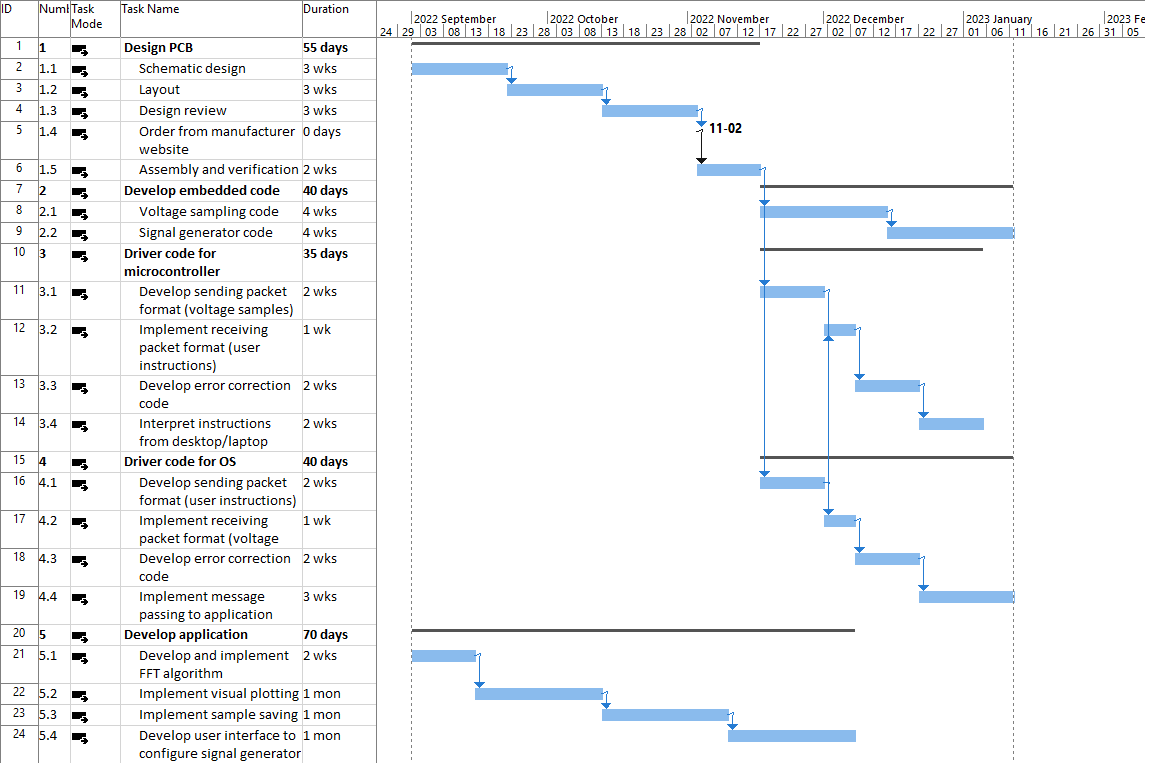
\includegraphics[height=14.5cm]{figures/gantt}
    \caption{Gantt chart displaying the breakdown and timing of project tasks.}
    \label{fig:gantt}
\end{figure}
\vfill
\raisebox{-0pt}{\makebox[\linewidth]{\thepage}}
\end{landscape}

\section{Test Plan}
\subsection{Printed Circuit Board (PCB)} % Ethan
The table below outlines the planned test cases for the PCB and the requisite
test result.

\begin{table}[h!]
    \centering
    \caption{Table of PCB test cases and the expected result.}
    \begin{tabularx}{\textwidth}{X|X}
        Description & Expected Result \\ 
        \hline
        \textbf{Case 1:} Probe the power and ground nets on the PCB using a
        continuity checker to ensure there are no shorts. & No continuity
        between power and ground. \\
        \hline
        \textbf{Case 2:} Connect the PCB to power via the USB port. & Power LED
        should turn on and there should be no short circuiting.\\
        \hline
        \textbf{Case 3:} Connect a JTAG debugger to the PCB & Microcontroller
        shows up in the JTAG chain of the debugger interface. \\
        \hline
        \textbf{Case 4:} Flash firmware to the MCU & Effect of running firmware is observed (Ie.
        blinking LED). \\
        \hline
        \textbf{Case 5:} Connect the signal generator output of the TeachEE to
        the voltage input and emit a waveform from the signal generator. & The
        same waveform is sampled properly and observed at the voltage input.
        Success in this test covers the function of both the ADC and DAC on the
        MCU.\\
    \end{tabularx}
\end{table}
\FloatBarrier

\noindent
The following subsections describe debugging actions that can be pursued if a
specific test case fails.

\subsubsection{Case 1}
If Case 1 has failed, there is a connection between power and ground. In this
case, the short circuit is present even when the device does not have power
indicating that the two nets are physically connected somewhere. The debugging
process will consist of checking for soldering and component orientation errors.

\subsubsection{Case 2}
If Case 2 fails, then the short circuit is only triggered on power up. Debug
this by looking for components that behaved as open circuits when powered off
but behave as shorts when powered on. Look for components that are producing
heat. Heat radiating off a certain part indicates that the short current is
flowing through it.

\subsubsection{Case 3}
If Case 3 fails, Then the debugger is not detecting the MCU it is connected to.
Check the physical connections to the debugger and ensure they are secure. Check
that the debugger is functioning properly by connecting it to another MCU that
is known to be working. Check that the MCU is powered properly. Check that the
supply voltage from the debugger is being used and not another power supply (too
much deviation from the logical voltage level of the debugger may create
connection issues).

\subsubsection{Case 4}
If Case 4 fails, then the debugger has established a connection but was unable
to flash firmware. Check the physical connections to the board. Check the data
rate and try slowing it down. Check the boot mode and reset pins of the MCU and
cross reference the datasheet to ensure they are in the correct state for JTAG
debugging.

\subsubsection{Case 5}
If Case 5 fails, then there could either be a hardware issue with the ADC or DAC
or a software issue with how they were configured. Start by using a secondary
oscilloscope to check that the signal is being outputted properly from the DAC.
If it is not, revise the software configuration. Once the DAC is functional,
check that the signal is arriving correctly at the ADC input. If no signal is
being read into the MCU's memory, then revise the software configuration to
handle this.

\subsection{Device Driver (OS Level)} % John

\subsubsection{Case 1}

A randomly generated message will be sent from the driver to the computer. The
message will then be manually verified for equivalence. The same will be
completed from the computer to the driver.

\subsubsection{Case 2}

A known message with an incorrect checksum should be sent from the computer to
the device. The device should detect the error, and apply the proper error
correction procedure. The same will be completed from the device to the
computer.

\subsubsection{Case 3}

A simulated disconnection of the device should occur at critical times of the
application process. This will ensure the proper handling of a sudden
disconnect.

\subsection{Application} % Eric
The desktop application takes voltage/time values and user inputs as input. The
outputs are plots of voltage vs time and voltage vs frequency, a CSV file
containing displayed information, and signal generator settings. \\

\noindent
To test the FFT algorithm, a unit testing framework, such as Google Test, can be
used. Test cases will contain various kinds of voltage/time inputs and their
corresponding expected outputs. Running the tests will automatically compare the
actual and expected outputs and indicate whether the tests passed or failed. The
input and output from each test case will be obtained by using an existing FFT
implementation. \\

\noindent
Waveform plotting will be manually verified to be correct by supplying a set of
test voltage/time values and observing the resulting waveform. A correct display
will show a stable waveform with horizontal and vertical scale adjusted based on
the test inputs. \\

\noindent
Sample saving will be tested by manually checking the CSV file for some test
data when the ``export'' button is clicked. Correctness can be verified by
checking that the displayed data is in the same range as the exported data and
that the voltage vs time and voltage vs frequency data present in the CSV file
match the data displayed on the waveforms. \\

\noindent
Verifying that signal generator settings are outputted correctly can be done by
supplying the parameters in the text boxes and ensuring that the values entered
by the user match the data sent to the OS side driver.

\section{Team} % Each person gets to write about themselves haha
The team consists of 3 members: John, Eric, and Ethan. Each team member's
competencies and role in the project are enumerated in the following
subsections.

% Discuss here why we divided it up the way we did.
\subsection{John}
John is a Computer Engineering student responsible for communication between the
device and the desktop application. This includes defining a protocol which
supports the transfer of sample data, and miscellaneous device configuration
signals. He will write the driver which allows the OS to communicate with the
device, and encapsulate it for easy use in the desktop application.

\subsection{Eric}
Eric is a Computer Engineering student and will be responsible for working on
the desktop application and message passing to the OS side driver. He is chosen
for this role because he has experience with C++ and OS-level development from
coursework and work experience, with an upcoming internship on virtual machine
development. He also has experience working with GUI frameworks in C++. 

\subsection{Ethan}
Ethan is a Computer Engineering student who will be managing and executing the
hardware side of the project. This role is defined as designing and testing the
PCB and configuring the development environment for John and Eric to use. Ethan
is selected for this role because he has worked in circuit design on internships
and has taken the computer hardware stream within ECE. Ethan also has software
engineering experience from internships and will be assisting wherever possible
in the software development process.

\section{Project Management Software} % John
The project's code will be hosted on a private GitHub repository. This will
allow for collaboration despite team members being in different locations or
timezones. Github also provides a robust issue system; a member can outline a
bug, labelled with a priority, and assign it to the respective member. A pull
request can be made once the issue has been resolved.\\

\noindent
Our team will follow an Agile Development Methodology, with a focus on frequent
short meetings, and with no members being restricted to a specific scope. This
will work well since the team is small and competent, which complements a
development style that is relatively flexible and unstructured.

% I left out jira because it doesn't make sense to use both jira and gh issues.
% Both can do backlogging, assigning to members, etc, etc.

\section{Deliverables}
% Try to underscope here as much as possible
% MVP plan
The deliverables listed in the following subsections are representative of the
prototype the team will be developing in ELEC 490. If a prototype of this scope
is completed sooner than expected then the team will begin work on some of the
planned features listed in Section \ref{sec:beyond}.

\subsection{Hardware}
% Ethan
% Single voltage in channel and signal gen
% bandwidth limit to whatever MCU is actually capable of
% Discuss code preprogrammed on the microcontroller?
The initial hardware prototype will be limited to a single voltage input and
signal generator output. These limitations match existing lab kits after
discussions with ECE professors and will minimize hardware complexity. The
bandwidth limitations of the device will be bounded by sample rate and
filtering. Following discussion with Dr. Whitehall, it was determined that a
sample rate amounting to 20 samples per period will ensure a correct waveform
with some interpolation. Most of the MCU options have ADCs with 1-2MSps.
Assuming 1MSps, the initial prototype will achieve a bandwidth of 50Khz.
Assuming an equal sample playback rate on the DAC, the signal generator will
produce up to 50Khz waveforms. Filtering could also limit bandwidth. The TeachEE
will use a Low Pass Filter (LPF) defined entirely in software. The software
defined LPF will allow users to adjust the characteristics of their sampling
setup in the laboratory. However, this data pre-processing will tax the Digital
Signal Processor (DSP) unit on the MCU and potentially slow down sample
throughput. This issue can likely be mitigated by iterating on the filter
design.

\subsection{Software} % Eric
% Basic GUI that plots the data
% Lets the user adjust signal gen settings
% Export to CSV for excel analysis
The final product will consist of a software package that users can install on
their desktop or laptop computer. It will feature the driver code for the
sending and receiving of data on the OS side and the frontend desktop
application. The application will feature a graphical user interface that plots
the received voltage samples as well as allowing users to adjust the PCB's
signal generator settings and export test results as a CSV. These are the
minimum deliverables for the project; future iterations of the project may add
more user functionality to the application.

\section{Beyond ELEC 390/49X} \label{sec:beyond} % John
% What we will work on if we meet the deliverables listed in prior section
% early

% Make GUI platform agnostic via web UI with SSO integration. This would allow students to save their data and access it from other devices while also having easy access to previous labs they have done.
% Second hardware prototype with external ADC and DAC to push better signal gen and bandwidth specs

Technology is inherently iterative, with TeachEE being no exception. The
following includes the most useful features that exist outside the minimum
viable product's scope, which should still be considered prior to the product's
launch, should one occur.

\subsection{Self Validation}

There should exist a mode that tests the entire pipeline, from the device to the
application. The device would generate a known signal, which is then sampled. If
the sample is outside of an acceptable range, an error should be displayed. The
sampled data could then be echoed back to the device via the computer to detect
error in the device's connection. The application could also verify that the
graphics are displayed correctly onto the screen by checking for suitable
overlap with a simulated waveform.

\subsection{Signal Preset Support}

A professor should be able to specify a signal via a user interface and export
the signal's specifications to a file. A student should then be able to load the
signal as a preset, and select a preset to be used by the device's signal
generator. This would decrease the time spent on application specific interface
details, and free up time for learning.

\subsection{Cloud Support}

A user's sampled data and presets should be synced via a user account. This
should be organizable via compartmentalizing into different labs and courses.
This would require extensive database and cloud development, and an extension of
the existing user interface onto web browsers. 

\subsection{Higher-Quality Tier}

There should exist a more-expensive version of the device which includes better
components. Different ADC and DAC components would give better sample rates and
bit-depths. This version should include more leads to sample more signals
concurrently. It must have a more aesthetically pleasing enclosure as well.

\subsection{Cross-platform Expansion}

The minimum viable product is required to function on a minimum of one platform.
When it is being developed, a cross platform framework is not guaranteed to be
selected. If this is the case, then some sections may need to be re-written in
different frameworks. This would include the device drivers, which are typically
written such that they are dependent on the operating system and hardware.

\newpage
\bibliographystyle{IEEEtran}
\bibliography{./report}
\end{document}